\documentclass[10pt,a4paper]{article}
\usepackage[margin=18mm]{geometry}
\usepackage[T1]{fontenc}
\usepackage{lmodern,graphicx,booktabs,amsmath,amssymb,array}
\usepackage[hidelinks]{hyperref}
\setlength{\parindent}{0pt}
\setlength{\parskip}{5pt}
\begin{document}
{\Large\bfseries Explicit functions for the actual degree-four transfer}\par
{\large\bfseries Weighted fibres, Hermite sections and complete local evaluation}\par
24 November 2026 \quad crypto PR5103 \quad [pcc:unverified]

\textbf{Result.} The genuine global map $f_4(P)=L([P-P_-])$ on the
actual genus-three curve now has explicit quartic/sextic rational
functions, a complete elliptic polynomial identity, and an evaluator
that resolves every rational basepoint. Equality with the actual map
uses global section existence and a degree bound, beyond finite-table
agreement. Native E/F and partial Lean G pass; the full geometry remains
a written proof with named inherited unsigned hypotheses.

\[
\begin{split}
 C/\mathbb F_7:\quad &X^4+4XY^3+2Y^4+5X^2Z^2+6XYZ^2+2Y^2Z^2+Z^4=0,\\
 E/\mathbb F_7:\quad &v^2=u^3+2u+6,\qquad R=(3,5).
\end{split}
\]
The full pole fibre of $g=f_4-R$ is
$D=(1:2:6)+(1:3:3)+2(1:5:5)$.
For $y=Y/X,z=Z/X$, put $q=1-z+yz$. Then
\[
g=(p_4/q^2,p_6/q^3),\qquad f_4=g+R,
\]
\[
\begin{aligned}
p_4={}&3+4z+4z^3+3z^4+5y+6yz+yz^2+yz^3\\
     &+3y^2+6y^2z+4y^2z^2+4y^3,\\[2pt]
p_6={}&6+z+3z^3+2z^4+2z^5+6yz+yz^2+3yz^3+4yz^4+2yz^5\\
     &+4y^2+5y^2z+4y^2z^2+2y^2z^3+3y^2z^4\\
     &+y^3+5y^3z+3y^3z^2+4y^3z^3.
\end{aligned}
\]
Homogenize $q,p_4,p_6$ to degrees $2,4,6$. Every coefficient and quotient
in $p_6^2-p_4^3-2p_4q^4-6q^6=F_CQ_8$ is retained in the full native output.

\begin{center}
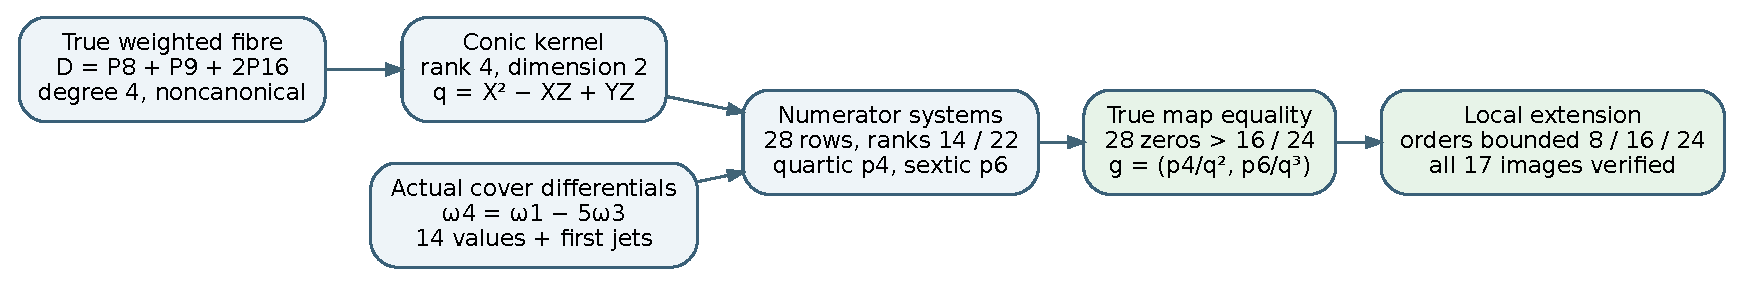
\includegraphics[width=\linewidth,height=49mm,keepaspectratio]{proof.pdf}
\end{center}

\textbf{Why this is the actual map.} The full weighted fibre and
noncanonical class give a two-dimensional conic kernel. The chosen
nonzero $q$ has $\operatorname{div}(q)\geq D$, so the already existing
true sections $x(g)q^2,y(g)q^3$ lie respectively in $H^0(C,\mathcal O_C(4))$ and $H^0(C,\mathcal O_C(6))$.
The plane hypersurface sequence and $H^1(\mathbb P^2,\mathcal O(m))=0$
give polynomial representatives. The actual integral $3L$ identity
gives $\omega_4=\omega_1-5\omega_3$ in characteristic seven. At all
14 nonpole points, values and first derivatives agree. A difference
section would have at least 28 zeros, exceeding degrees 16 or 24.
Thus both sections coincide globally. Smoothness and properness extend
the fractions, retaining the actual geometric degree four. Proof b0036d.

\newpage
{\Large\bfseries Exact qualification, limits and next mechanism}\par

\textbf{Complete exceptional evaluation.} The polynomial-only evaluator
constructs the actual implicit curve series through $t^{24}$ and uses
leading coefficients. The historical image oracle enters only after
evaluation. Every one of the 17 rational images agrees after adding $R$.
\begin{center}
\begin{tabular}{clcl}
\toprule
Index & $C$ point & $(v(q),v(p_4),v(p_6))$ & $g$\\
\midrule
0 & $(1:0:1)$ & $(1,2,3)$ & $(5,1)$\\
8 & $(1:2:6)$ & $(1,0,0)$ & $O$\\
9 & $(1:3:3)$ & $(1,0,0)$ & $O$\\
11 & $(1:4:2)$ & $(1,2,3)$ & $(2,5)$\\
16 & $(1:5:5)$ & $(2,0,0)$ & $O$\\
\bottomrule
\end{tabular}
\end{center}
The nonzero section degrees bound all zero orders by 8,16,24, so the
truncation contains every leading coefficient. At $X=0$, $q=YZ$ and
the quartic forbids $YZ=0$; hence every geometric basepoint lies in
the implicit $X=1$ chart. This gives a complete local method over a
supplied field of definition. The implemented field and qualified
population are $\mathbb F_7$ only. Proof 73fe27.

\textbf{Native evidence.} E source~\texttt{5cd0a093}, data f062d9:
73 locked and 44 changed whole-file readbacks before calls, all seven
strict phases 0, guards unchanged, full 19267-byte stdout and 40 small
originals. F source~\texttt{d1a52ece}, data 5e0a6f: 89 locked and 12
changed whole-file readbacks, all seven phases 0, guards unchanged,
22726-byte stdout and 40 small originals. Pinned Rust1.99.1,
120 seconds/2 GiB/one worker, warnings errors, no suppressions.
Actual numerator, value-row and residual leading-coefficient mutations
reject; pristine restores. The residual mutant $(5,2)$ is not on $E$.

\textbf{Partial Lean arithmetic.} G source~\texttt{5bd2d8ca} had 102
locked and 60 changed whole-file readbacks. Lean4.35.0, Init only,
default logic and the same bounds: both phases 0, guards unchanged.
All 91 closed standard Int coefficient congruences print no axioms.
The full 7019-byte axioms output and 20 small originals are retained.
Data 5996b3 with appended count correction 485a0c. Native polynomial
expansion and written geometric bridges remain distinct; these are
not a full Polynomial, function-field or Jacobian formalization.

\textbf{Preserved negatives and alternate $S_4$ check.} There are zero
four-distinct rational fibres (A b4a734). The first B run failed raw
projective-representative equality; C normalized those same points and
checked all nine weighted pairs without changing the cohort. All first
failures remain. The complete $(2,1,1)$ fibre supplies tame transposition
inertia. With inherited geometric primitivity, only $A_4,S_4$ remain;
the transposition excludes $A_4$. The alternate proof 9a6918 preserves
the earlier cyclic/theta proof and its unsigned dependencies.

\textbf{Custody and CI.} Whole original E/F ELFs (4696712/4653896 bytes,
hash prefixes~\texttt{eacb59c4}/\texttt{5a82205f}) and G olean
(109840 bytes,~\texttt{bf79000f}) remain in RAM pending approved durable
custody. New focused CI artifacts cannot replace them. Parent5095 and
cryptanalysis1961 focused native/Lean jobs pass; other applicable checks,
stacked-parent requirements and the frozen main ledger fork remain holds.
No merge, rerun, waiver or independent signed scientific verdict is claimed.

\textbf{Next unblocked work.} Determine the exact canonical ramification
line from the actual differential, factor its full line-quartic section,
and evaluate any residual extension-field ramification points and branch
images. No factor pattern is assumed. This fixed small-field result
establishes no ECDLP advantage over rho/BSGS/index calculus, no
crypto-scale family and no proper-subfield descent from $\mathbb F_7$.
Exact proof maps, all sources/locks and inventories are in the study;
primary section/divisor references: Stacks01XS,0AYQ,02RS,0B5B.
All scientific standing remains [pcc:unverified].
\end{document}
